\chapter{Approach}

\section{Planing of the movement}

The movement is planed as multiple stages.
\begin{itemize}
	\item The robot shall find the PegBoard
	\item The robot shall itentify the correct pins
	\item The robot shall pick up a pin
	\item The robot shall place a pin in a different hole
\end{itemize}

\subsection{First Stage: Where is the PegBoard}

In the first stage the robot arm uses the camera located on the end-effector in order to find the board.
The board is indicated by a landmark at the corner of the board.

\begin{figure}[H]
    \begin{center}
        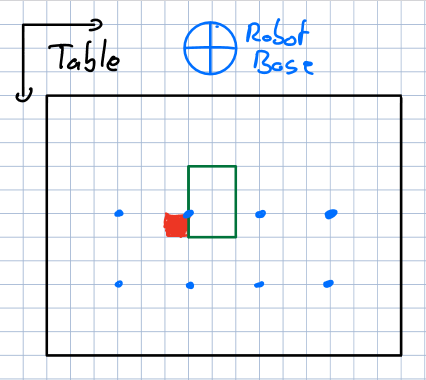
\includegraphics[width=0.3\linewidth]{images/MovementStep1.png}
        \caption{Planing phase}
    \end{center}
\end{figure}

This figure shows a schematic representation of the table where the robot works on.
The green box is the peg board.
The red square is the landmark and the blue dots are points on the table
where the robot is looking for the landmark on the table.
Sawyer starts looking for a landmark in the lower left corner and then proceeds from left to right and from down to top.

When a landmark is found the robot stops searching for the pegboard
and uses the position of the landmark as a reference point for the the pegboard.
